
Here we study invariants of two well-known Circumhyperbolae\footnote{Its centers lie in the unshaded regions in Figure~\ref{fig:midlines}.}: the Feuerbach and Jerabek Hyperbolas $F$ and $J$ \cite[Jerabek Hyperbola]{mw}. Both are rectangular since they contain $X_4$ \cite{mw}. The former is centered on $X_{11}$ and the latter on $X_{125}$. With respect to 3-periodics no invariants have been detected for $J$. However, the Jerabek $J_{exc}$ of the Excentral Triangle, which passes through the Excenters and is centered on $X_{100}$\footnote{The Excentral's $X_{125}$ \cite{mw}.}, does produce interesting invariants\footnote{The Feuerbach Hyperbola $F_{exc}$ has not yet yielded any detectable invariants over the 3-periodic family.}. 
$F$ is known to pass through $X_1$ and $X_9$ of its reference triangle. Interestingly
$J_{exc}$ also passes through $X_1$ and $X_9$. This stems from the fact that $J$ passes through $X_4$ and $X_6$. Since the Excentral Triangle is always acute \cite{coxeter67}, its $X_4$ is $X_1$. Likewise, the excentral $X_6$ is $X_9$. 

The Isogonal Conjugate of a Circumconic is a line \cite[Circumconic]{mw}. Remarkably:

\begin{remark}
The Isogonal conjugate of $F$ with respect to a reference triangle and that of $J_{exc}$ with respect to the Excentral one is line $X_1X_3=\mathcal{L}_{650}$.
\end{remark}

The first part is well-known \cite[Feuerbach Hyperbola]{mw}. For the second part, consider that $J$ is the Isogonal Conjugate of the Euler Line \cite[Jerabek Hyperbola]{mw}. The Euler Line of the Excentral Triangle passes through its $X_4$ and $X_5$ which are $X_1$ and $X_3$ in the reference 3-periodic.

Referring to Figure~\ref{fig:circumhyps}:

\begin{proposition}
$J_{exc}$ intersects $E_9$ in exactly two locations.
\end{proposition}

\begin{proof}
Let $s_i,i=1,2,3$ refer to 3-periodic sidelengths. The perspector of $J_{exc}$ is $X_{649}=s_1(s_2-s_3)::$ (cyclical) \cite{etc}. Therefore the trilinears $x:y:z$ of $J_{exc}$ satisfy \cite{yiu2003}:
 \[J_{exc}: {s_1(s_2-s_3)}x^2+s_2(s_3-s_1)y^2+s_3(s_1-s_2)z^2=0.\]
 
Notice the above is satisfied for the Excenters $[1:1:-1],\; [1:-1:1]$ and $ [-1:1:1]$. As $X_1=[1:1:1]$ and $X_9=s_2+s_3-s_1::$ (cyclical) it follows that
 $J_{exc}(X_1)=J_{exc}(X_9)=0$.
 
 Eliminating variable $x$, the intersection of $J_{exc}=0$ and $E_9=0$ is given by the quartic:
 
 \begin{align*}
 &s_2(s_1-s_3)k_1 y^4+2s_2(s_1-s_3){k_1}{k_2}y^3 z\\
 +&2s_3(s_1-s_2){k_1}{k_2}y z^3+s_3(s_1-s_2)k_1 z^4=0
 \end{align*}
 
With $k_1=(s_1+s_2-s_3)^2$ and $k_2=s_1+s_3-s_2$. The discriminant of the above equation is:
 
 \[
 -432[(s_2-s_3)(s_1-s_3)(s_1-s_2)(s_1+s_3-s_2)^2(s_1-s_2-s_3)^2(s_1+s_2-s_3)^2(s_1s_2s_3)]^2
 \]
 
Since it is negative, there will be two real and two complex solutions \cite{burnside_1960}.
\end{proof}



\begin{proposition}
$F$ intersects the $X_9$-centered Circumellipse at $X_{1156}$.
\end{proposition}

\begin{proof}
The perspector of $X_9$ is $X_1$ and that of $X_{11} $ is $X_{650}=(s_3-s_3)(s_3+s_3-s_1)::$ (cyclical). Therefore, the trilinears $x:y:z$ of $F$ and $E_9$ satisfy:

\begin{align*}
    F:&(s_2-s_3)(s_2+s_3-s_1)/x+\\
    &(s_3-s_1)(s_3+s_1-s_2)/y+\\
    &(s_1-s_2)(s_1+s_2-s_3)/z=0 \\
    E_9:& 1/x+1/y+1/z=0.
\end{align*} 

$X_{1156}$ is given by $1/[(s_2-s_3)^{2}+s_1( s_2+s_3-2s_1)]::$ (cyclic). This point can be readily checked to satisfy both of the above.
\end{proof}
 
 %abaixo: nao e a Jerabek do excentral e sim do bilhar
%The intersection of $E_9$ with the Jerabek circumhyperbola %$J$ is given by the point
%$X^*=[g(a,b,c):g(b,c,a):g(c,a,b)]$ where
%$g(a,b,c)=(b+c)(a^4 - ( b^2-bc+c^2)a^2-bc(b-c)^2)$. 

Given a generic triangle $T$, the following two claims are known:

\begin{proposition}
The asymptotes of both $F$ and $J_{exc}$ are parallel to the $X_9$-centered circumconic, i.e., $c_4$ and $c_5$ in \eqref{eqn:e0} vanish.
\end{proposition}

\begin{proof}
To see the first part, consider that since the Caustic is centered on $X_9$ and tangent to the 3-periodics, it is the (stationary) Mandart Inellipse $I_9$ of the family \cite{mw}. This inconic is known to have axes parallel to the asymptotes of $F$ \cite{gibert2004-mandart}. Since the Caustic is confocal with the EB, $F$ asymptotes must be parallel to the EB axes.

Secondly, 3-periodics are the Orthic Triangles of the Excentrals, therefore the EB is the (stationary) Excentral's Orthic Inconic \cite{mw}. The latter's axes are known to be parallel to the asymptotes of the Jerabek hyperbola. \cite[Orthic Inconic]{mw}.

An alternate, algebraic proof appears in Appendix \ref{app:circum-x1x2x9}.
\end{proof}

\noindent Let $\lambda$ (resp. $\lambda'$) be the focal length of $F$ (resp. $J_{exc}$).

\begin{remark}
Isosceles 3-periodics have $\lambda'=\lambda=0$.
\end{remark}

To see this consider the sideways isosceles 3-periodic with $P_1=(a,0)$. $P_2$ and $P_3$ will lie on the 2nd and 3rd quadrants at $(-a_c,{\pm}y')$, where $a_c=a(\delta-b^2)/(a^2-b^2)$ is the length of the Caustic major semi-axis \cite{garcia2020-ellipses}. $X_1$ and $X_4$ will lie along the 3-periodic's axis of symmetry, i.e., the x-axis. To pass through all 5 points, $F$ degenerates to a pair of orthogonal lines: the x-axis and the vertical line $x=-a_c$. The foci will collapse to the point $(-a_c,0)$. A similar degeneracy occurs for the upright isosceles, i.e., when $P_1=(0,b)$, namely, the foci collapse to $(0,-b_c)$, where $b_c=b(a^2-\delta)/(a^2-b^2)$ is the Caustic minor semi-axis length.

\begin{theorem}
For all non-isosceles 3-periodics, $\lambda'/\lambda$ is invariant and given by:
\label{thm:focal-ratio}
\end{theorem}
 
\begin{equation}
 \frac{\lambda'}{\lambda}= \frac{\sqrt{\delta^2+\left(a^2+b^2\right)\delta+ a^2b^2}}{a b}=\sqrt{2/\rho}>2
 \label{eqn:focal-ratio}
\end{equation}

\begin{proof}
Assume the EB is in the form of \eqref{eqn:billiard-f}. Let the 3-periodic be given by $P_i=(x_i,y_i),i=1,2,3$. $F$ passes through the $P_i$, $X_1$ and $X_9=(0,0)$. The asymptotes of $F$ are parallel to the EB axes, therefore this hyperbola is given by $c_1x+c_2y+c_3 x y = 0$ and $\lambda^2=|8c_1c_2/c_3^2|$, where: 
\begin{align}
c_1=& y_2y_3(x_2-x_3)x_1^2+(x_2^2y_3-x_3^2y_2-y_2^2y_3
+y_2y_3^2)x_1y_1 \nonumber\\
+&y_2y_3(x_2-x_3)y_1^2  
-(x_2y_3-x_3y_2)(x_2x_3+y_2y_3)y_1
 \nonumber \\
 c_2=&x_2x_3(y_2-y_3)x_1^2+(x_2x_3^2-x_2^2x_3-x_2y_3^2+x_3y_2^2)x_1y_1 \label{eqn:ci} \\
 +&(x_2y_3-x_3y_2)(x_2x_3+y_2y_3)x_1-x_2x_3(y_2-y_3)y_1^2 \nonumber\\
 c_3=& (x_2y_3-x_3y_2)x_1^2+
(x_3^2y_2-x_2^2y_3+  y_2^2y_3-y_2y_3^2)x_1 \nonumber\\
+&(x_3y_2-x_2y_3 )y_1^2 
+(x_2^2x_3-x_2x_3^2+x_2y_3^2-x_3y_2^2)y_1 \nonumber
\end{align}
 
Let $P_i'=(x_i',y_i'),i=1,2,3$ be the Excenters. They are given by
\begin{align} 
    P_1'=&\left({\frac {-{x_1}\,{s_1}+{x_2}\,{s_2}+{x_3}\,{s_3}}{{
s_2}+{s_3}-{s_1}}},{\frac {-{y_1}\,{s_1}+{y_2}\,{
s_2}+{y_3}\,{s_3}}{{s_2}+{s_3}-{s_1}}}\right) \nonumber\\
P_2'=& \left({\frac {{x_1}\,{s_1}-{x_2}\,{s_2}+{x_3}\,{s_3}}{{
s_3}+{s_1}-{s_2}}},{\frac {{y_1}\,{s_1}-{y_2}\,{
s_2}+{y_3}\,{s_3}}{{s_3}+{s_1}-{s_2}}}\right) \label{eqn:pi-prime} \\
P_3'=& \left({\frac {{x_1}\,{s_1}+{x_2}\,{s_2}-{x_3}\,{s_3}}{{
s_1}+{s_2}-{s_3}}},{\frac {{y_1}\,{s_1}+{y_2}\,{
s_2}-{y_3}\,{s_3}}{{s_1}+{s_2}-{s_3}}}\right) \nonumber
\end{align}
Here, $s_1=|P_2-P_3|$, $s_2=|P_1-P_3|$ and $s_3=|P_1-P_2|$.

Since $J_{exc}$ is also centered on the origin and has horizontal/vertical asymptotes, $J_{exc}$ is given by $c_1'x+c_2'y+c_3'x y=0$, and $(\lambda')^2=|8c_1'c_2'/(c_3')^2|$, where $c_i'$ are constructed as \eqref{eqn:ci} replacing $(x_i,y_i)$ with $(x_i',y_i')$.

Consider a right-triangle\footnote{We found this to best simplify the algebra.} 3-periodic, e.g., with $P_1$ at $(x^\perp,y^\perp)$ given in \eqref{eqn:perp} and $P_2$ and $P_3$ obtained explicitly \cite{garcia2019-incenter}. From these obtain $c_i$ using \eqref{eqn:ci}. Using \eqref{eqn:pi-prime} obtain $P_i'$ and the $c_i'$. Finally, obtain a symbolic expression for $\lambda'/\lambda$. After some manipulation and simplification with a Computer Algebra System (CAS), we obtain \eqref{eqn:focal-ratio} which we call a {\em candidate}.

Parametrize the 3-periodic family with $P_1(t)=(a\cos{t},b\sin{t})$ and using the sequence above arrive at an expression for $\lambda'/\lambda$ in terms of $t$. Subtract that from the right-triangle candidate. After some algebraic manipulation and CAS simplification verify the subtraction vanishes, i.e., $\lambda'/\lambda$ is independent of $t$.
\end{proof}

\begin{figure}
    \centering
    \includegraphics[width=\textwidth]{pics_eps_new/0060_circumhyps.eps}
    \caption{An $a/b=1.5$ EB is shown (black) as well as a sample 3-periodic (blue), the confocal Caustic (brown), and the Excentral Triangle (green). The 3-periodic's Feuerbach Circumhyperbola $F$ (orange) passes through its three vertices as well as $X_1$, $X_9$, and $X_4$. The Excentral's Jerabek Circumhyperbola $J_{exc}$ (purple) passes through the three Excenters, as well as $X_1$, $X_9$ and $X_{40}$ (not shown). Two invariants have been detected over the orbit family: (i) the asymptotes (dashed) of both $F$ and $J_{exc}$ stay parallel to the EB axes, (ii) the ratio of focal lengths is constant (focal axis appears dashed). $F$ intersects the Billiard at $X_{1156}$.}
    \label{fig:circumhyps}
\end{figure}

\subsection{Focal Length Extrema}

Let $P_1(t)=(a\cos{t},b\sin{t})$. While their ratio is constant, $\lambda$ and $\lambda'$ undergo three simultaneous maxima in $t\in(0,\pi/2)$, see Figure~\ref{fig:focal-ratio}. In fact, the following additional properties occur at configurations of maximal focal length (we omit the rather long algebraic proofs), see Figure~\ref{fig:zero-hyps}:

\begin{itemize}
    \item $F'$ is tangent to the Caustic at ${\pm}X_{11}$.
    \item $J'_{exc}$ is tangent to the EB at ${\pm}X_{100}$, i.e., at ${\mp}X_{1156}$ (see below).
    %\item $k'_J=a/b$.
\end{itemize}

\begin{remark}
Like $F$, $J'_{exc}$ intersects the EB at $X_{1156}$.
\end{remark}

This happens because $X_{1156}$ is the reflection of $X_{100}$ about $X_9$. If the latter is placed on the origin, then $X_{1156}=-X_{100}$, and $J'_{exc}$ passes through ${\pm}X_{100}$.

Let $F'$ and $J'_{exc}$ be copies of $F$ and $J_{exc}$ translated by $-X_{11}$ and $-X_{100}$ respectively, i.e., they become concentric with the EB (focal lengths are unchanged). Since their asymptotes are parallel to the EB axes and centered on the origin, their equations will be of the form:

\[
F': x\,y = k'_F,\;\;J'_{exc}: x\,y = k'_J
\]

\begin{remark}
$\lambda=2\sqrt{2k'_F}$, $\lambda'=2\sqrt{2k'_J}$, $\lambda'/\lambda=\sqrt{k'_J/k'_F}=\sqrt{2/\rho}$.
\end{remark} 

\begin{figure}
    \centering
    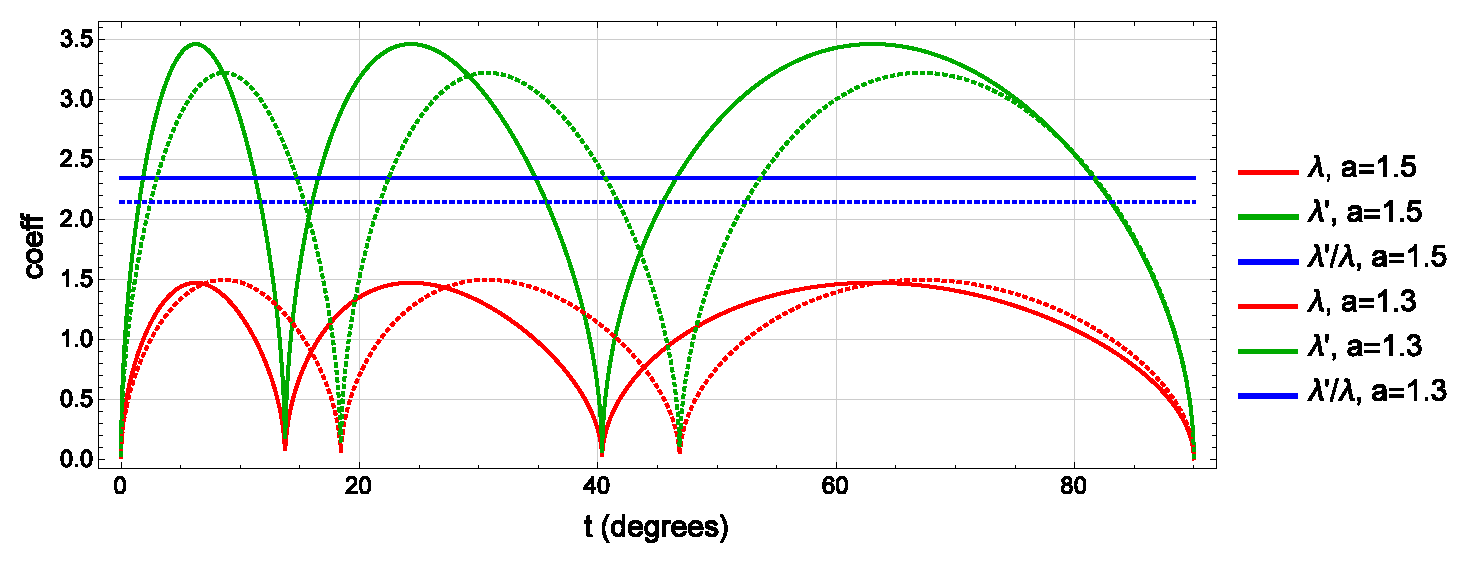
\includegraphics[width=\textwidth]{pics_eps_new/0110_hyp_focals.eps}
    \caption{Focal lengths $\lambda,\lambda'$ of $F,J_{exc}$ vs the parameter $t$ in $P_1(t)=(a\cos{t},b\sin{t})$ are shown red and green. The solid (resp. dasheD) curves correspond to $a/b=1.5$ (resp. $a/b=1.3$). In the first quadrant there are 3 maxima. $\lambda'/\lambda$ (blue) remain constant for the whole interval.}
    \label{fig:focal-ratio}
\end{figure}

\begin{figure}
    \centering
    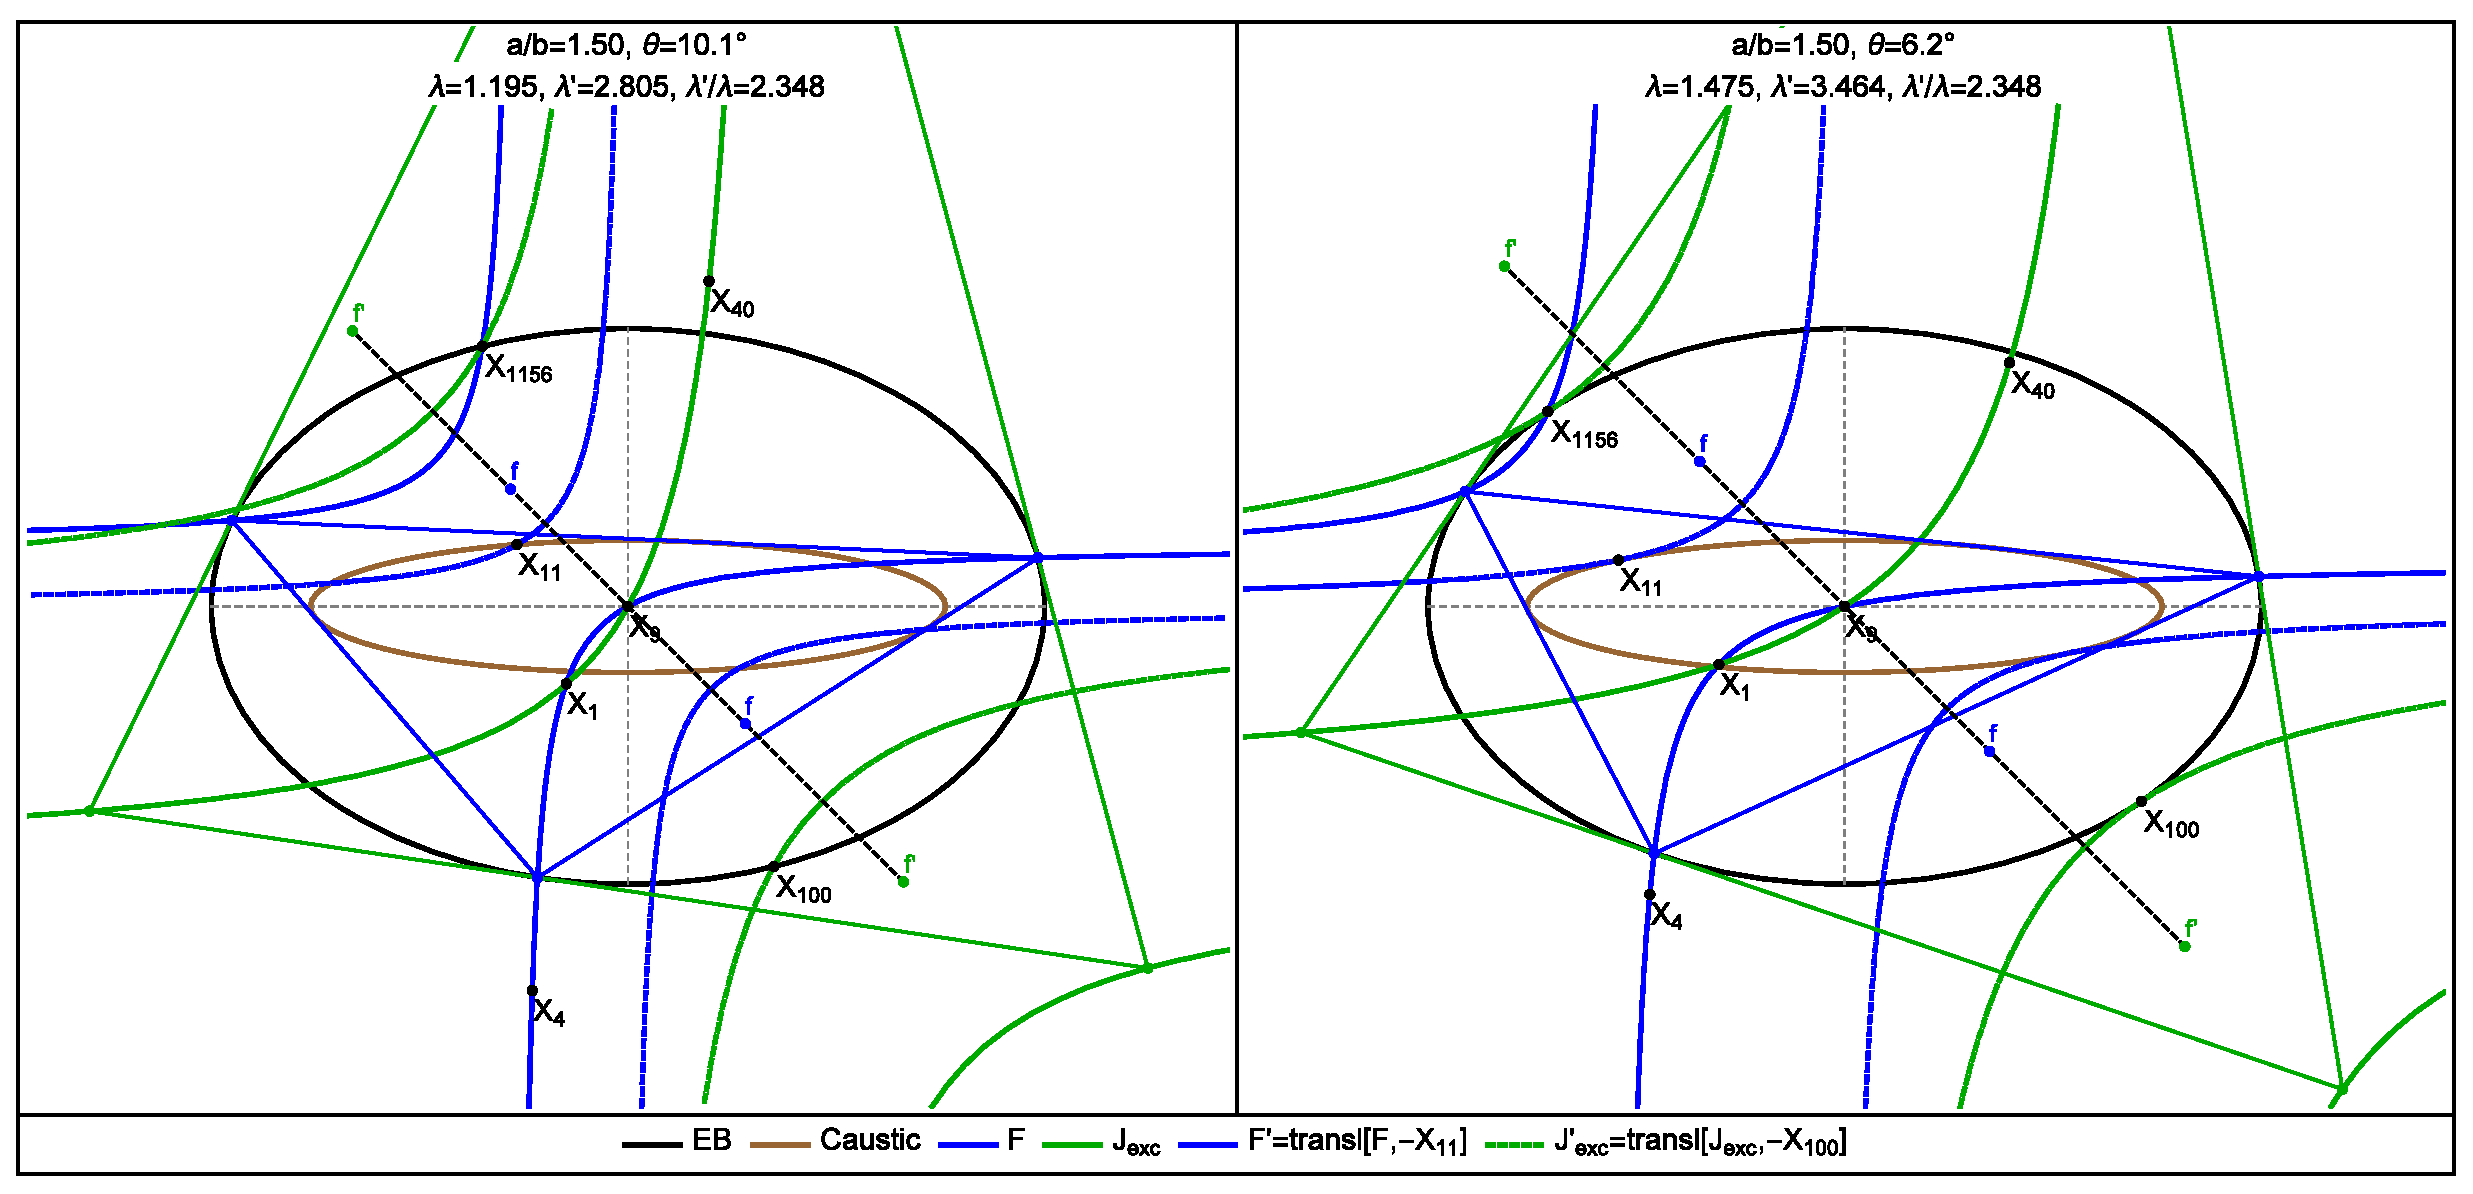
\includegraphics[width=\textwidth]{pics_eps_new/0100_zero_hyps.eps}
    \caption{Two snapshots of $J$ and $F_{exc}$ drawn solid blue and solid green, respectively, for $a/b=1.5$. Also shown (dashed) are copies $F'$ and $J'_{exc}$ of both hyperbolas translated so they are dynamically concentric with the EB (translate $J$ by $-X_{11}$ and $F_{exc}$ by $-X_{100}$). Their focal lengths $\lambda,\lambda'$ are identical to the original ones; their focal axes are collinear and shown the dashed diagonal through the EB center. Notice that like $F$, $J'$ also intersects the EB at $X_{1156}$. \textbf{Left}: $t=10.1^\circ$, showing an intermediate value of ether focal length. \textbf{Right}: $t=6.2^\circ$, focal lengths are at a maximum. When this happens, the translated copy of $F$ (resp. $J_{exc}$) is tangent to the Caustic (resp. EB) at $X_{11}$ (resp. $X_{1156})$. \textbf{Video}: \cite[PL\#09,10]{reznik2020-playlist-circum}}
    \label{fig:zero-hyps}
\end{figure}

\